\newpage
\section{Generator}
The purpose of this block is to convert rotational energy into electrical energy. Once converted, the electrical energy can be deposited in the Load System.

As the Generator was chosen by the customer and as it is pre-mounted on the Roll Stand, the block will not be designed but will be analysed instead.

\subsection{Implementation}
The Generator consists of a DC-motor which is mounted on the Roll Stand. The motor's rotor connected with a drive shaft through a gearing. This drive shaft runs through the Torque Sensor and connects with the Roll - which in turn can be rotated by a car (AU2). \fxnote{omformulering af sætning efter bndestreg - TN}

\begin{figure}[H]
	\centering
	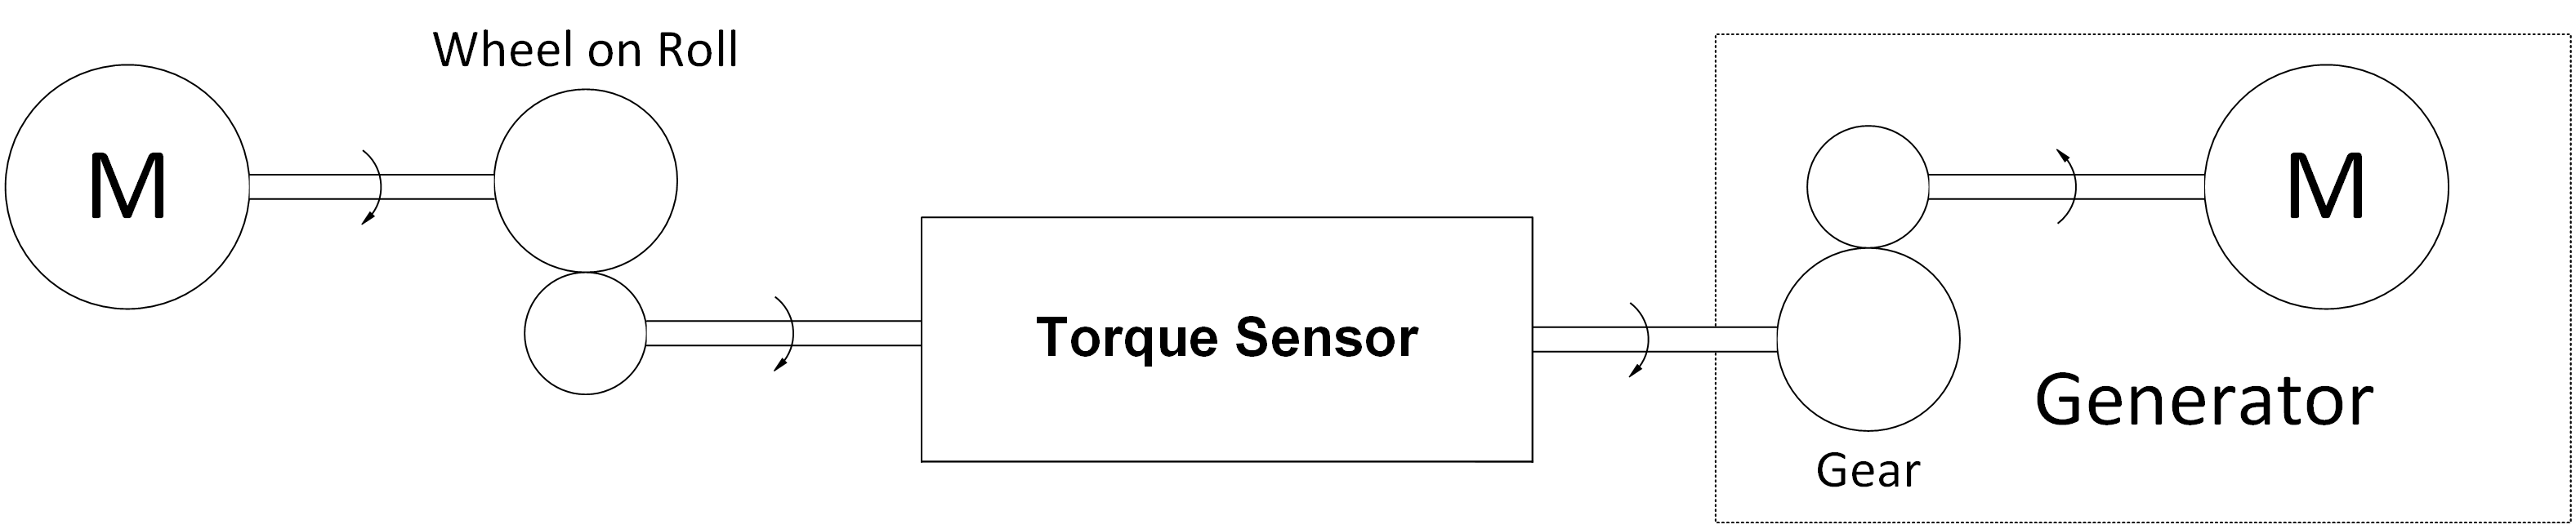
\includegraphics[width=1\linewidth]{Hardware/Pictures/Mechanical_Connections}
	\caption{Mechanical configuration in the Roll Stand}
	\label{fig:Generator_Implementation}
\end{figure}

\subsection{Analysis}
\label{sec:GeneratorAnalysis}
The Generator is built with a MAXON 200 Watt DC-motor with permanent magnets\cite{Maxon}. When the motor's rotor is spun, a voltage drop will be created between the motor's positive and negative terminals. The voltage-drop depends on the the motor velocity constant k\textsubscript{e} which for the specified motor is given as:
\begin{equation}
	K_e = 248 \frac{rpm}{V} = \SI[per-mode=fraction]{25.97}{\radian \per \second \per \volt}
\end{equation}

The maximum possible voltage-drop between the Generator's terminals, when AU2 is tested with Rolling Road, can be calculated by using the cruise speed (maximum velocity) of AU2\cite{BAC_zenith33}. It is given as:
\begin{equation}
	v_{wheel} = \SI[per-mode=fraction]{30}{\meter \per \second}
\end{equation}

Due to the difference in diameter between AU2's wheel and the Roll creates a gearing ratio R\textsubscript{1} between the wheel's and the generator's angular velocity. This ratio can be determined by the diameters of the wheel and the Roll:
\begin{equation}
	\begin{split}
		d_{wheel} &= \SI{478}{\milli \meter}\\
		d_{Roll} &= \SI{152}{\milli \meter}\\
		\\
		R_1 &= \frac{d_{wheel}}{d_{Roll}} = \frac{478 mm}{152 mm} = 3.15
	\end{split}
\end{equation}

As seen on Figure \vref{fig:Generator_Implementation}, another gearing is installed between the Torque Sensor's output and the Generator's input. This ratio is given as:
\begin{equation}
	R_2 = 1:4.3 = 0.233
\end{equation}

The wheel's angular velocity, when AU2 runs at cruise speed, can be calculated using the velocity and the radius of the wheel:
\begin{equation}
	\omega_{wheel} = \frac{v_{wheel}}{r_{wheel}} = \frac{v_{wheel}}{d_{wheel} \cdot 0.5} = \frac{\SI[per-mode=fraction]{30}{\meter \per \second}}{\SI{152}{\milli \meter} \cdot 0.5} = \SI[per-mode=fraction]{34.87}{\radian \per \second}
\end{equation}

The angular velocity of the Roll then be found using the gearing ratio between the wheel and the Roll (it is assumed that there is no slip between them):
\begin{equation}
		\omega_{Roll} = \omega_{wheel} \cdot R_1 = \SI[per-mode=fraction]{34.87}{\radian \per \second} \cdot 3.15 = \SI[per-mode=fraction]{109.65}{\radian \per \second}
\end{equation}

Angular velocity of the Generator's rotor:
\begin{equation}
		\omega_{rotor} = \omega_{Roll} \cdot R_2 = \SI[per-mode=fraction]{109.65}{\radian \per \second} \cdot 0.233 = \SI[per-mode=fraction]{471.49}{\radian \per \second}
\end{equation}

The stationary value of the induced voltage-drop between the Generator's terminals at AU2's cruise speed can then be calculated as:
\begin{equation}
		V_b = \frac{\omega_{rotor}}{k_e} = \frac{\SI[per-mode=fraction]{471.49}{\radian \per \second}}{\SI[per-mode=fraction]{25.97}{\radian \per \second \per \volt}} = \SI{18.16}{\volt}
\end{equation}

\subsection{Unit test}
The Generator hasn't had a unity \fxnote{Det er nok bare at referere til den anden test -JH}test since this was done in the Previous System\cite{BAC_rullefelt} and the system implemented in Rolling Road is identical. For a complete unit test of the Generator, the reader is referred to the related documentation on page 74 to 77.